\documentclass[letterpaper]{article}


\PassOptionsToPackage{numbers}{natbib}
\usepackage[preprint]{neurips_2023}
\usepackage[utf8]{inputenc} % allow utf-8 input
\usepackage[T1]{fontenc}    % use 8-bit T1 fonts
\usepackage{hyperref}       % hyperlinks
\usepackage{url}            % simple URL typesetting
\usepackage{booktabs}       % professional-quality tables
\usepackage{amsfonts}       % blackboard math symbols
\usepackage{nicefrac}       % compact symbols for 1/2, etc.
\usepackage{microtype}      % microtypography
\usepackage{xcolor}         % colors
\usepackage{tikz}
\usepackage{pgfplots}
\usepackage{tabularx,ragged2e}
\usepackage{amsmath}
\usepackage{subcaption}



\newcolumntype{L}{>{\RaggedRight}X}
\pgfplotsset{width=10cm,compat=1.9}


%%%%%%%%%%%%%%%%%%%%%%%%%%%%%%%%%%%%%%%%%%%%%%%%%%%%%%%%%%%%


\title{Generalizable IC Routing using Deep RL with a GNN-based Policy Network}

\author{%
    Roozmehr Jalilian, Bruce Xi \\
    Department of Electrical \& Computer Engineering \\
    The University of British Columbia \\
    \texttt{\{roozmehr.jalilian,xsd99\}@ece.ubc.ca} \\
    Vancouver, BC V6T 1Z4 }


\begin{document}


\maketitle


\begin{abstract}
Routing in integrated circuits (IC) design is often modeled as a pathfinding
problem and has consistently represented one of the most challenging aspects due
to its complexity and time-consuming nature. Even with state-of-the-art
commercial CAD tools, routing complex designs can take hours, if not days.
Consequently, there is a growing interest in applying machine learning-based
approaches to overcome these challenges. In previous work, we introduced a novel
reinforcement learning (RL) approach for routing. While this RL router
outperformed the baseline, it was limited by poor generalizability, requiring a
new policy to be trained from scratch for each problem. In this project, we aim
to address this limitation by introducing a novel graph neural network (GNN) as
the policy network for the RL router. This enhancement allows the agents to
generalize their learned routing policies to new, unseen designs, reducing the
computation time significantly.
%TODO: Briefly mention the results that we've obtained (if it helps, that is!).
\end{abstract}

\section{Introduction}
Physical design is a crucial phase in the IC design process, wherein the logical
representation of the chip is converted into a physical geometric layout
essential for fabrication foundries. This stage is subdivided, with routing
being a key step were pins specified by netlists are connected using wires and
vias. The quality of the routing, often evaluated by wirelength and egde
overflow, impacts vital chip metrics like performance, power, and area
\cite{Hu2001}.

For 2-dimensional circuit layouts, routing can be modeled as a pathfinding
problem in a 2D grid, where the objective is to establish paths connecting pins
placed on different coordinates of the said grid. This grid can be treated like
a graph, with the circuit's pins placed on its nodes and the connections between
them occupying its edges. Each edge possesses a capacity feature, indicating the
maximum number of permissible wires due to the physical constraints of wire
thickness and finite space within a chip region. An optimal routing solution
seeks to minimize total wire length and avoid edge overflow (usage of an edge
exceeding its capacity), ensuring all connections are efficient and within
capacity.

Two important terminologies here are net and netlist. A {\it net} refers to a
set of pins requiring connection, and a {\it netlist} is a set consisting of
multiple nets that need routing during the process. For clarity, we will use the
terms {nodes} and {pins} interchangeably throughout this paper.

Complexities of traditional routing algorithms have inspired researchers to
use machine-learning-based techniques instead. One such technique is
RL, and specifically, its deep variant (DRL), which is
a fusion of RL and deep neural networks. It has showcased capabilities exceeding
human performance in various contexts \cite{mnih2013playing}.

In prior research, we introduced a multi-agent RL router to address the IC
routing challenge. Each agent, tasked with routing one individual net, operated
concurrently under a shared super policy, as we designed the agents to be
homogeneous and fully-cooperative. Trained with proximal policy optimization
(PPO) \cite{Schulman2017} and evaluated against benchmarks, this RL router
demonstrated superior performance compared to the A* baseline. However, a
limitation emerged: the policy, though effective for specific benchmarks, lacked
generalizability for other, albeit similar, problems. We attributed this
shortfall to the policy neural network's architecture, comprising a multilayer perceptron (MLP), which struggled to extract rich information from the
state encodings.

Contrastingly, GNNs exhibit robust generalization
capabilities when processing graphical data \cite{Almasan2022,Wang2018},
aligning with the routing problem’s grid graph model. In this project, we
introduce a novel message-passing GNN architecture integrated into the RL
router’s policy and value networks. The GNN accepts the routing grid graph from the
environment as state input and determines actions accordingly. This innovation
aims to bolster the RL router’s ability to generalize trained policy to problems
not encountered during training, promising substantial reductions in computation
time.


\section{Related work}
Numerous studies in existing literature have verified the effectiveness of
employing GNNs within the policy/value network of
RL models to enhance generalization, especially when
the agent’s environment is graph-representable. However, to our knowledge, no
existing study has directly explored the use of GNN equipped RL for IC routing.

For instance, \cite{Liao2020} introduced an RL IC router trained via a Deep
Q-Network (DQN), utilizing an MLP as the RL agent's
value network. However, similar to our previous work, it showed a lack of
generalization. \cite{liao2020attention} proposed an attention-based RL router,
which was built on top of a genetic algorithm (GA) router. Although the authors
claimed it had significant performance and generalization capabilities, it was
only compared against the very GA router that acted as its baseline, and the
performance gain could only be described as marginal.

Contrastingly, \cite{Almasan2022} incorporated a GNN as the value network of an
RL agent, also trained by DQN. This approach manifested notable generalization
capabilities in network routing—a field bearing similarities to IC routing—and
serves as the principal inspiration for this paper. In parallel, both
\cite{Chen2023} and \cite{Wang2018} echoed the integration of GNNs with RL
models wherein the operational problems are graphs. Furthermore,
\cite{Mirhoseini2021} and \cite{Yue2022} adopted GNNs as encoder layers for
their respective RL policy and value networks. \cite{Cheng2021} introduced a
hybrid RL agent, which was designed to solve both IC placement and routing
simultaneously. The authors incorporated both CNN and GNN models in the policy
network of their RL agent to capture as much information about the netlists as
possible; however, their methodology put more focus on placement than routing,
and they didn't evaluate their agent in terms of generalizability.

    
\section{Methodology}

\subsection{IC routing as a pathfinding problem}
\autoref{fig:grid} illustrates a simplified IC routing problem, framed as a pathfinding task on a grid graph. The objective is to route a net between two pins at coordinates (0,0) and (3,3). Each edge in this graph has a capacity of one, indicating that it can be traversed no more than once. The challenge, therefore, lies in finding the shortest path between these points while adhering to the edge traversal constraints.

\begin{figure}[h!]
    \centering
    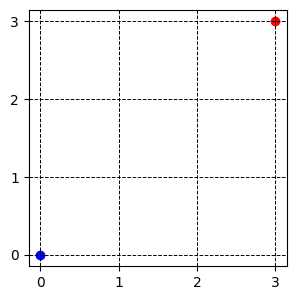
\includegraphics[width=0.3\textwidth]{figure/grid_grap.png}
    \caption{The grid graph of a simple IC routing problem.}
    \label{fig:grid}
\end{figure}

\subsection{GNN-based RL framework for IC routing}
An illustration of the proposed RL routing framework is displayed in \autoref{fig:overview}. The framework involves an agent engaging repeatedly with an environment. At each time step \(t\), the agent is presented with an observation \(S_{t}\) and a reward \(R_{t}\), and then at the subsequent time step, \(t+1\), it executes an action \(A_{t+1}\) in the environment. This process is directed by a policy network and a value network. The policy network approximates the policy \(\pi_{\theta_1}(a|s) = P(A_{t+1}=a|S_{t}=s)\), signifying the probability of choosing action \(a\) given the environment is in state \(s\). This function is represented by the proposed GNN, parameterized by \(\theta_1\), which will be detailed later. The value network approximates the value function \(V_{\theta_2}(s)\) and is instrumental in updating the policy network's parameters \(\theta_1\). It employs a similar GNN architecture as the policy network but operates with distinct parameters, ensuring \(\theta_1 \neq \theta_2\).

\begin{figure}[h!]
    \centering
    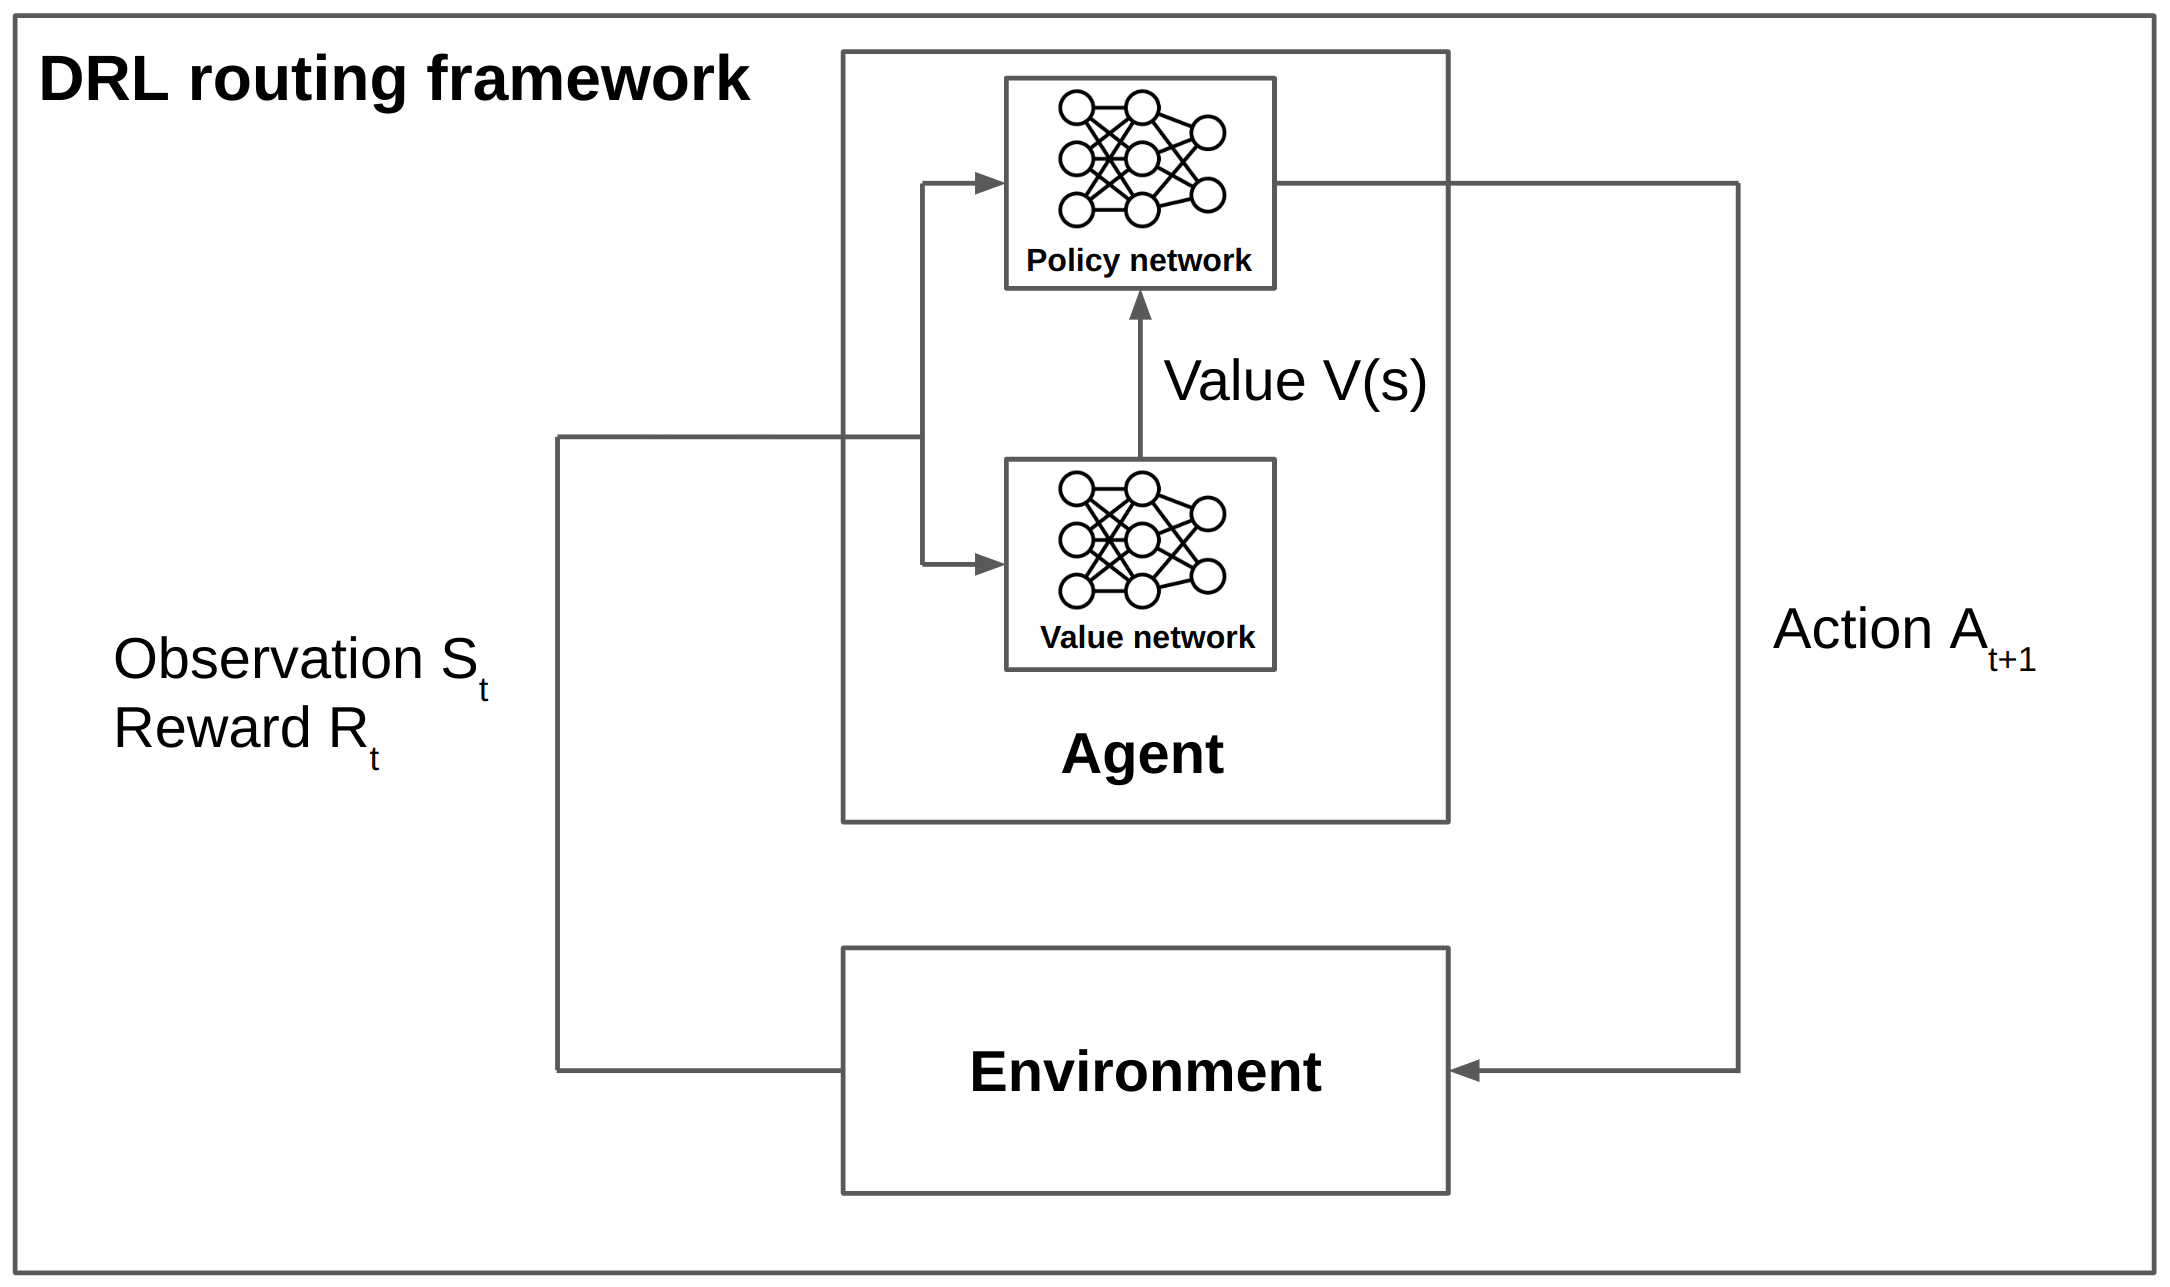
\includegraphics[width=\textwidth]{figure/overview.png}
    \caption{The overview of the proposed DRL routing framework.}
    \label{fig:overview}
\end{figure}


\subsection{Environment}
The environment encapsulates the grid pathfinding problem. It processes actions from the agent, updates its internal states, and subsequently provides new observation states and rewards to the agent.
\subsubsection{Observations}
Observations are the states discernible by an agent from the environment, containing essential details about the environment. These include a node feature matrix \(\mathbf{X} \in \mathbb{R}^{N \times 2}\), an edge feature matrix \(\mathbf{E} \in \mathbb{R}^{N \times N}\), and an adjacency matrix \(\mathbf{A} \in \mathbb{R}^{N \times N}\). In a grid comprising \(N\) nodes, each node is represented by a 2D feature vector \(x\), with both elements being binary. The first element, \(x_1\), signifies that the agent is currently at this node if it equals 1, while \(x_2\) denotes the target position. The matrix \(\mathbf{E}\) holds the scalar capacity of each edge, which decreases by 1 each time the agent traverses a specific edge.


%TODO: demonstration

\subsubsection{Reward Function}
The environment imposes a -1 penalty on the agent for each step taken not leading to the target, thereby incentivizing the discovery of the shortest path. Successfully reaching the target, characterized by the agent and target occupying the same node, grants a +100 reward. This event is indicated when a vector \(x\) in \(\mathbf{X}\) has both elements equal to 1. The reward function \( R(\mathbf{X}) \) is defined as:
\begin{equation}
    R(\mathbf{X}) = \begin{cases} 
    100 & \text{if } \exists i \in \{1, 2, \ldots, N\}, x_{i_1} = x_{i_2} = 1, \\
    -1 & \text{otherwise}.
    \end{cases}
\end{equation}
This reward structure encourages the agent to minimize wirelength, synonymous with the distance traveled to reach the target. Any unnecessary deviations result in reduced cumulative rewards.

\subsection{Agent}
The agent, upon receiving observations and rewards from the environment, inputs these into the policy and value networks. The former generate probability distributions of actions. During training, the parameters of these networks are optimized to produce a sequence of actions that maximizes cumulative reward.

\subsubsection{Actions}
Actions within this framework are represented by integers ranging from 0 to 3, corresponding to the agent moving up, right, down, or left from its current position via an edge. Following each action, the environment transitions to a new state, resulting in updates to \(\mathbf{E}\) and \(\mathbf{X}\).

\subsubsection{GNN Design}
The Graph Neural Network (GNN) utilizes \(\mathbf{A}\), \(\mathbf{E}\), and \(\mathbf{X}\) as inputs. Initially, it encodes the node feature matrix \(\mathbf{X}\) into a hidden representation matrix \(\mathbf{H^t}\). This process is represented as:
\begin{equation}
    h_i^0 = F_{\text{encode}}(x_i)
\end{equation}
where \(F_{\text{encode}}\) is an MLP. The superscript \(t\) in \(\mathbf{H}\) denotes the number of message-passing iterations. At the outset, when no message passing has occurred, \(t=0\). 

The subsequent step involves computing messages for each node, formulated as:
\begin{equation}
    m_{ji} = F_{\text{message}}([h_j^t, h_i^t, e_{ji}])
\end{equation}
Here, \(F_{\text{message}}\) is another MLP. The vector \([h_j^t, h_i^t, e_{ji}]\) is a concatenation of the hidden states \(h_j^t\) and \(h_i^t\) from \(\mathbf{H^t}\), and the scalar capacity \(e_{ji} \in \mathbf{E}\) of the edge connecting nodes \(i\) and \(j\). The third step aggregates messages for each node from all neighboring nodes:
\begin{equation}
    \bar{m}_{i} = \sum_{j \in N_{\text{in}}} m_{ji}
\end{equation}
The aggregated message \(\bar{m}_{i}\) for node \(i\) is the sum of messages received from all its \(N_{\text{in}}\) neighbors. The fourth step updates the hidden states of all nodes using their current states and aggregated messages:
\begin{equation}
    h_{i}^{t+1} = F_{\text{update}}(h_{i}^t, \bar{m}_{i})
\end{equation}
In this step, \(F_{\text{update}}\) is implemented using a gated recurrent unit (GRU). The message-passing process, encompassing steps 2 to 4, is repeated \(T\) times, where \(T\) is the diameter of the input grid graph.

The final step involves reading out the policy logits for the policy network, or the value for the value network. The policy logits are then passed through a softmax layer to obtain the probability distribution of actions. This step aggregates all node states \(h_i^T\) and forwards the result to another MLP for further processing.


\subsection{Training}
The proposed GNN is integrated into our RL routing framework, acting as both the policy and value network. Training is conducted using PPO \cite{Schulman2017} with RLlib. The GNN's parameters are optimized through stochastic gradient descent, influenced by the feedback from the value network.

\section{Experiments}
An MLP-based RL framework serves as a baseline for comparing the performance of our GNN-based RL network. Both frameworks underwent 40 training iterations with benchmark A. Following this, three evaluations were carried out:

(1) Policies trained with benchmark A were tested on the same benchmark to compare the performance and training efficiency between GNN and MLP.

(2) Zero-shot policies from benchmark A, were applied on benchmark B to assess the generalizability of the two frameworks. Details of these benchmarks are provided in the subsequent table.

(3) The policies were further trained on benchmark B for an additional 40 iterations (fine-tuning). The performances of GNN and MLP during fine-tuning were then compared.

\begin{table}[h!]
    \caption{Two benchmarks used for training and testing.}
    \centering
    \begin{tabularx}{\textwidth}{LLL}
        \toprule
        Parameter & Benchmark A & Benchmark B \\
        \midrule
        Length & 4 & 4 \\
        Width & 4 & 4 \\
        Source node coordinates & (0,0) & (3,0) \\
        Target node coordinates & (3,2) & (0,1) \\
        Edge capacity & 2 & 2 \\
        \bottomrule
    \end{tabularx}
\end{table}

\subsection{Comparing training efficiency}
\autoref{fig:training} displays the training efficiencies (reward versus training iteration) of both the GNN and MLP-based frameworks. Notably, the GNN-based framework demonstrates an ability to attain a higher reward after 40 iterations of training. \autoref{fig:inference} illustrates the routing solutions generated by both frameworks. It is observed that each framework successfully identifies an optimal path between the source and the target node. This outcome is attributed to the simplicity of the benchmark. Consequently, it can be concluded that both GNN and MLP are capable of learning a policy from one benchmark, which then performs optimally when tested with the same benchmark utilized for training.

\begin{figure}[h!]
    \centering
    \begin{subfigure}[b]{0.45\textwidth}
        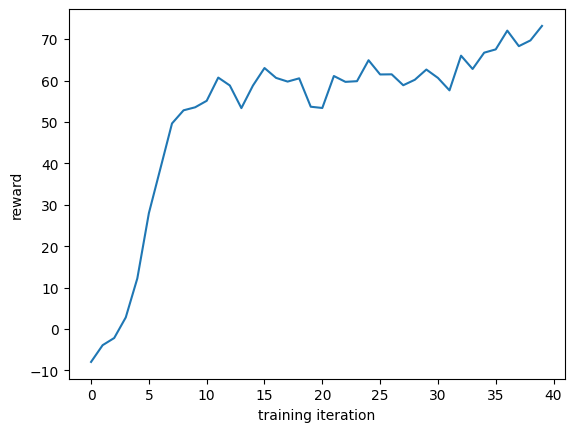
\includegraphics[width=\textwidth]{figure/gnn_training.png}
        \caption{}
    \end{subfigure}
    \begin{subfigure}[b]{0.45\textwidth}
        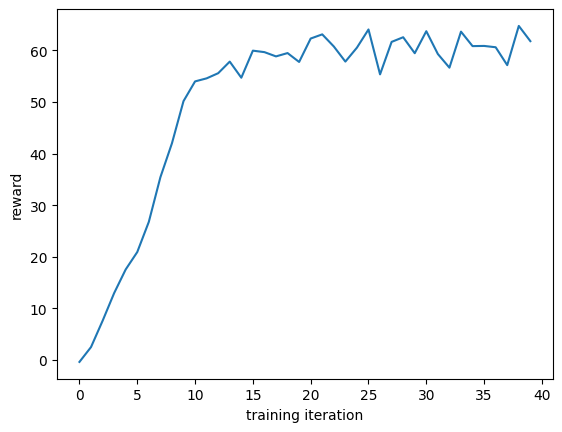
\includegraphics[width=\textwidth]{figure/mlp_training.png}
        \caption{}
    \end{subfigure}
    \caption{Training efficiencies for (a) GNN-based framework, (b) MLP-based framework.}
    \label{fig:training}
\end{figure}

\begin{figure}[h!]
    \centering
    \begin{subfigure}[b]{0.45\textwidth}
        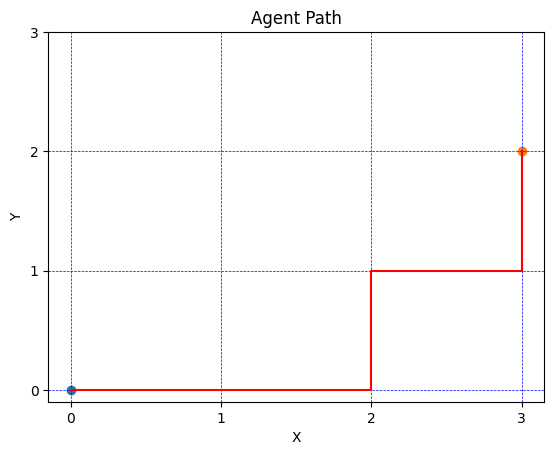
\includegraphics[width=\textwidth]{figure/gnn_inference.png}
        \caption{}
    \end{subfigure}
    \begin{subfigure}[b]{0.45\textwidth}
        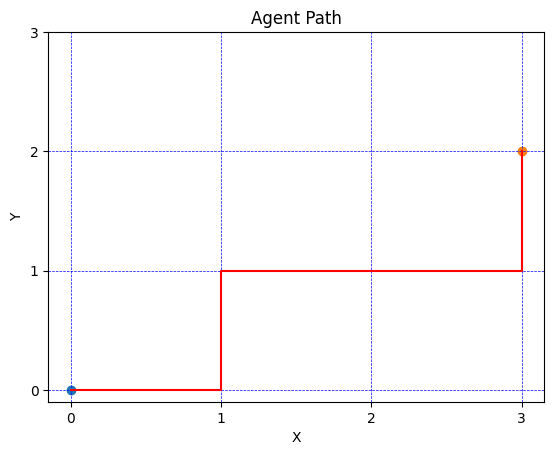
\includegraphics[width=\textwidth]{figure/mlp_inference.png}
        \caption{}
    \end{subfigure}
    \caption{Inference results for (a) GNN-based framework, (b) MLP-based framework on benchmark A.}
    \label{fig:inference}
\end{figure}

\subsection{Comparing zero-shot performance} \label{m:0} 
\autoref{fig:0shot} presents the zero-shot performance of both the GNN and MLP frameworks on benchmark B, utilizing policies acquired from benchmark A. The results indicate that neither framework is able to produce valid routing results, despite the benchmarks being quite similar and straightforward in nature. This leads to the conclusion that substituting MLP with GNN in the RL framework does not enhance its zero-shot generalizability.

\begin{figure}[h!]
    \centering
    \begin{subfigure}[b]{0.45\textwidth}
        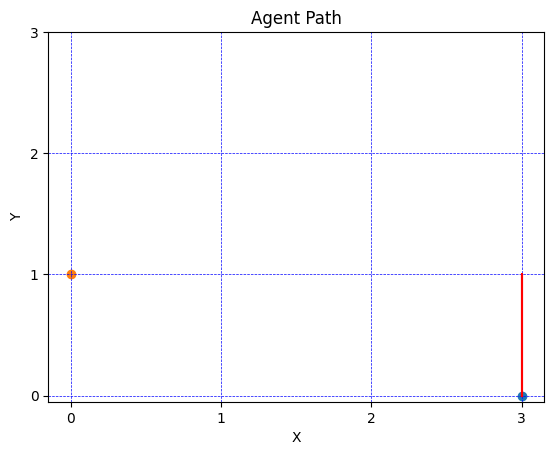
\includegraphics[width=\textwidth]{figure/gnn_0shot.png}
        \caption{}
    \end{subfigure}
    \begin{subfigure}[b]{0.45\textwidth}
        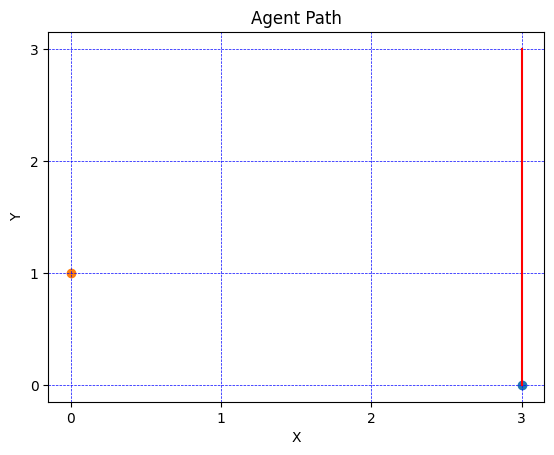
\includegraphics[width=\textwidth]{figure/mlp_0shot.png}
        \caption{}
    \end{subfigure}
    \caption{Zero-shot performance of (a) GNN-based framework, (b) MLP-based framework on benchmark B, using policies trained with benchmark A.}
    \label{fig:0shot}
\end{figure}

\subsection{Comparing fine-tuning performance}

\autoref{fig:ft} displays the fine-tuning outcomes for both RL agents. Unfortunately, due to issues originating from the RLlib library, neither agent could undergo effective fine-tuning when exposed to benchmarks different from those used in their initial training. This is evident from the reward versus time curves, which remain flat, signifying that the policy networks in both RL agents did not undergo any updates. Consequently, they remained in a static state, unable to adapt or improve.


\begin{figure}[h!]
    \centering
    \begin{subfigure}[b]{0.45\textwidth}
        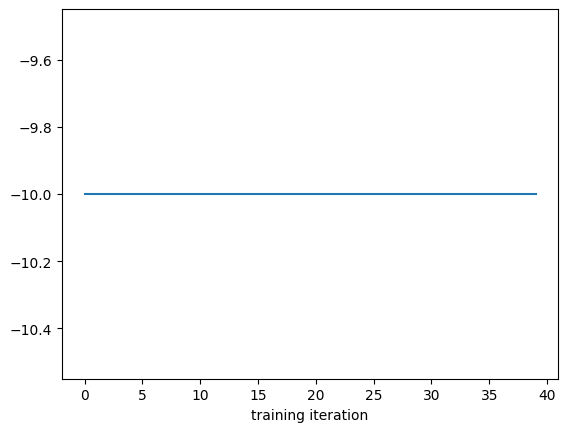
\includegraphics[width=\textwidth]{figure/fine_tuning.png}
        \caption{}
    \end{subfigure}
    \begin{subfigure}[b]{0.45\textwidth}
        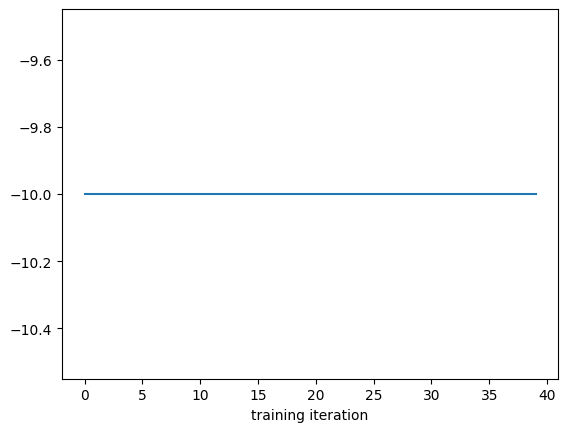
\includegraphics[width=\textwidth]{figure/fine_tuning.png}
        \caption{}
    \end{subfigure}
    \caption{Fine-tuning  of (a) GNN-based framework, (b) MLP-based framework on benchmark B, based on policies trained with benchmark A.}
    \label{fig:ft}
\end{figure}

\section{Conclusion}
In this project, a message-passing GNN is proposed for integration into an RL framework for IC routing. The aim is to enhance the generalizability of RL policies, allowing for policies trained in one environment to be effectively transferred to or fine-tuned for unseen environments. However, challenges such as implementation limitations and bugs in the RLlib library prevented the attainment of conclusive results. These issues underscore the need for future work, particularly in the manual development and implementation of the RL training policy, to re-evaluate the generalizability of the GNN-based RL framework.
%%%%%%%%%%%%%%%%%%%%%%%%%%%%%%%%%%%%%%%%%%%%%%%%%%%%%%%%%%%%
    
{
\small
\bibliographystyle{IEEEtranN}
\bibliography{references}
}

%%%%%%%%%%%%%%%%%%%%%%%%%%%%%%%%%%%%%%%%%%%%%%%%%%%%%%%%%%%%


\end{document}